\documentclass[a4paper,12pt]{article}
\usepackage{graphicx}
\begin{document}

\paragraph{Goal of the project} \hspace{0pt}
\\
\\
The goal is to make an optimized solution for finding the shortest path in a vector-based geometry. The program will assume that geometry is Euclidean, that way the shortest possible path between two points is assumed to be a straight line.
\\
\\
Instead of dividing the geometry into pixels, here points will be placed in a two-dimensional
coordinate, that will then be joined to form a chain of edges. Edges are then required to form
a loop - in other words - a shape. This shape can then be interpreted as a wall or a non-wall.
\\
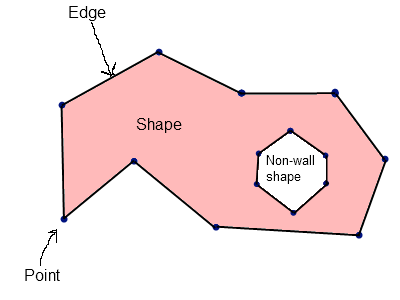
\includegraphics[scale=0.65]{pointedgeshape.png}
\\
Each point in the vector field is connected to two other points. That way each point can be considered as an angle between the non-wall part.
\\
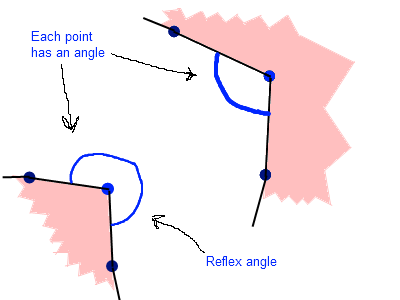
\includegraphics[scale=0.65]{pointsandangles.png}
\\
\\
Pathfinding algorithm generates the shortest available path from point A to point B,
avoiding possible walls along the way. Algorithm will construct a graph from the vector field.
All points whose angles are reflex (between 180$^\circ$ and 360$^\circ$) are vertices in the graph. Points A and B are vertices as well. Edges in the graph have a value, which is a distance between two vertices calculated with Pythagerous theorum. That way an edge value can't be less than zero. With this graph the shortest path between points A and B can be found using the Dijkstra's algorithm.
\\
\\
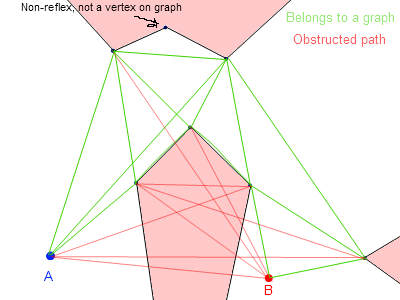
\includegraphics[scale=0.65]{graph.png}
\\
\\
Two points are connected in the graph if the path between these points is unobstructed.
Because of this the project will require a tracing algorithm. Current idea of the algorithm is taking each point and mapping a maximum distance for all of its directions.
\\
\\
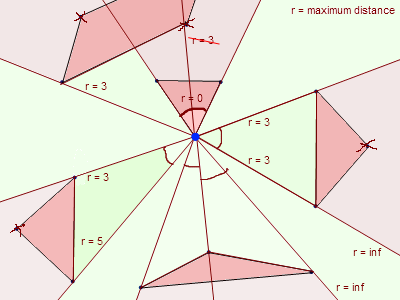
\includegraphics[scale=0.65]{trace.png}
\\
\\
The project will provide a relatively user-friendly tool for geometry manipulation. This tool will imitate a brush of a certain width, leaving a track with each stroke of a computer mouse. The stroke either creates a wall shape, or erases a piece of wall from the field. Straight-forward point manipulation via point dragging is provided as well.
\\
\\
Main focus in the project is on optimization. Pathfinding algorithm should work on run-time in
modern middle-end computers. Editing the vector field and repositioning the destination point
should work on run-time as well.

\end{document}